\documentclass{book}


\usepackage{graphicx}
\usepackage{moreverb}
\usepackage{amsmath}
\usepackage{alltt}
\usepackage{rotating}
\usepackage{subfigure}
\usepackage{toc}
\usepackage{xspace}

\newcommand{\extref}[1]{$\S$\ref*{#1}}   % No hyperlink. For external refs. \extref
\newcommand{\comma}{\> ,}
\newcommand{\period}{\> .}
\newcommand{\wt}{\widetilde}
\newcommand{\grv}{\textasciigrave}
\newcommand{\hyperbf}[1]{\textbf{\hyperpage{#1}}}
\newcommand{\Ss}{\(^*\)}
\newcommand{\Dd}{\(^\dagger\)}

\newcommand{\AND}{&& \hskip -17pt\relax}
\newcommand{\CR}{\\}
\newcommand{\CRNO}{\nonumber \\}
\newcommand{\dstyle}{\displaystyle}

\newcommand{\Begineq}{\begin{equation}}
\newcommand{\Endeq}{\end{equation}}
\newcommand{\NoPrint}[1]{}

\newcommand{\pow}[1]{\cdot 10^{#1}}
\newcommand{\Bf}[1]{{\bf #1}}
\newcommand{\bfr}{\Bf r}

\newcommand{\bmad}{{\sl Bmad}\xspace}
\newcommand{\tao}{{\sl Tao}\xspace}
\newcommand{\mad}{{\sl MAD}\xspace}
\newcommand{\cesr}{{\sl CESR}\xspace}

\newcommand{\sref}[1]{\S\ref{#1}}
\newcommand{\Sref}[1]{Sec.~\sref{#1}}
\newcommand{\cref}[1]{Chapter~\ref{#1}}

\newcommand{\Newline}{\hfil \\ \relax}

\newcommand{\eq}[1]{{(\protect\ref{#1})}}
\newcommand{\Eq}[1]{{Eq.~(\protect\ref{#1})}}
\newcommand{\Eqs}[1]{{Eqs.~(\protect\ref{#1})}}

\newcommand{\vn}{\ttcmd}           % For variable names
\newcommand{\vni}{\ttcmdindx}
\newcommand{\cs}{\ttcmd}           % For code source
\newcommand{\cmd}{\ttcmd}          % For Unix commands
\newcommand{\rn}{\ttcmd}           % For Routine names
\newcommand{\tn}{\ttcmd}           % For Type (structure) names
\newcommand{\bn}[1]{{\bf #1}}       
\newcommand{\toffset}{\vskip 0.01in}
\newcommand{\rot}[1]{\begin{rotate}{-45}#1\end{rotate}}

\newcommand{\data}{{\mbox{data}}}
\newcommand{\reference}{{\mbox{ref}}}
\newcommand{\model}{{\mbox{model}}}
\newcommand{\base}{{\mbox{base}}}
\newcommand{\design}{{\mbox{design}}}
\newcommand{\meas}{{\mbox{meas}}}
\newcommand{\var}{{\mbox{var}}}

\newcommand\ttcmd{\begingroup\catcode`\_=11 \catcode`\%=11 \dottcmd}
\newcommand\dottcmd[1]{\texttt{#1}\endgroup}

\newcommand\ttcmdindx{\begingroup\catcode`\_=11 \catcode`\%=11 \dottcmdindx}
\newcommand\dottcmdindx[1]{\texttt{#1}\endgroup\index{#1}}

\newcommand{\St}{$^{st}$\xspace}
\newcommand{\Nd}{$^{nd}$\xspace}
\newcommand{\Th}{$^{th}$\xspace}
\newcommand{\B}{$\backslash$}
\newcommand{\W}{$^\wedge$}

\newcommand{\cbar}[1]{\overline C_{#1}}

\newlength{\dPar}
\setlength{\dPar}{1.5ex}

\newenvironment{example}
  {\vspace{-3.0ex} \begin{alltt}}
  {\end{alltt} \vspace{-2.5ex}}

\newcommand\Strut{\rule[-2ex]{0mm}{6ex}}

\newenvironment{Itemize}
  {\begin{list}{$\bullet$}
    {\addtolength{\topsep}{-1.5ex} 
     \addtolength{\itemsep}{-1ex}
    }
  }
  {\end{list} \vspace*{1ex}}

\newcommand{\Section}[1]{\section{#1}\indent\vspace{-3ex}}

\newcommand{\SECTION}[1]{\section*{#1}\indent\vspace{-3ex}}

% From pg 64 of The LaTex Companion.

\newenvironment{ventry}[1]
  {\begin{list}{}
    {\renewcommand{\makelabel}[1]{\textsf{##1}\hfil}
     \settowidth{\labelwidth}{\textsf{#1}}
     \addtolength{\itemsep}{-1.5ex}
     \addtolength{\topsep}{-1.0ex} 
     \setlength{\leftmargin}{5em}
    }
  }
  {\end{list}}


\setlength{\textwidth}{6.25in}
\setlength{\oddsidemargin}{0.25in}
\setlength{\evensidemargin}{0.00in}
\setlength{\textheight}{8.5in}
\setlength{\topmargin}{0in}

\begin{document}

%----------------------------------------------------------------
% Cover Page

\thispagestyle{empty}

\begin{flushright}
\large
  Revision: 0.1 \\
  9 June, 2004 \\
\end{flushright}

\vfill

{
\begin{center}
{\Huge \sf\bf The} \\
\vskip 0.1in
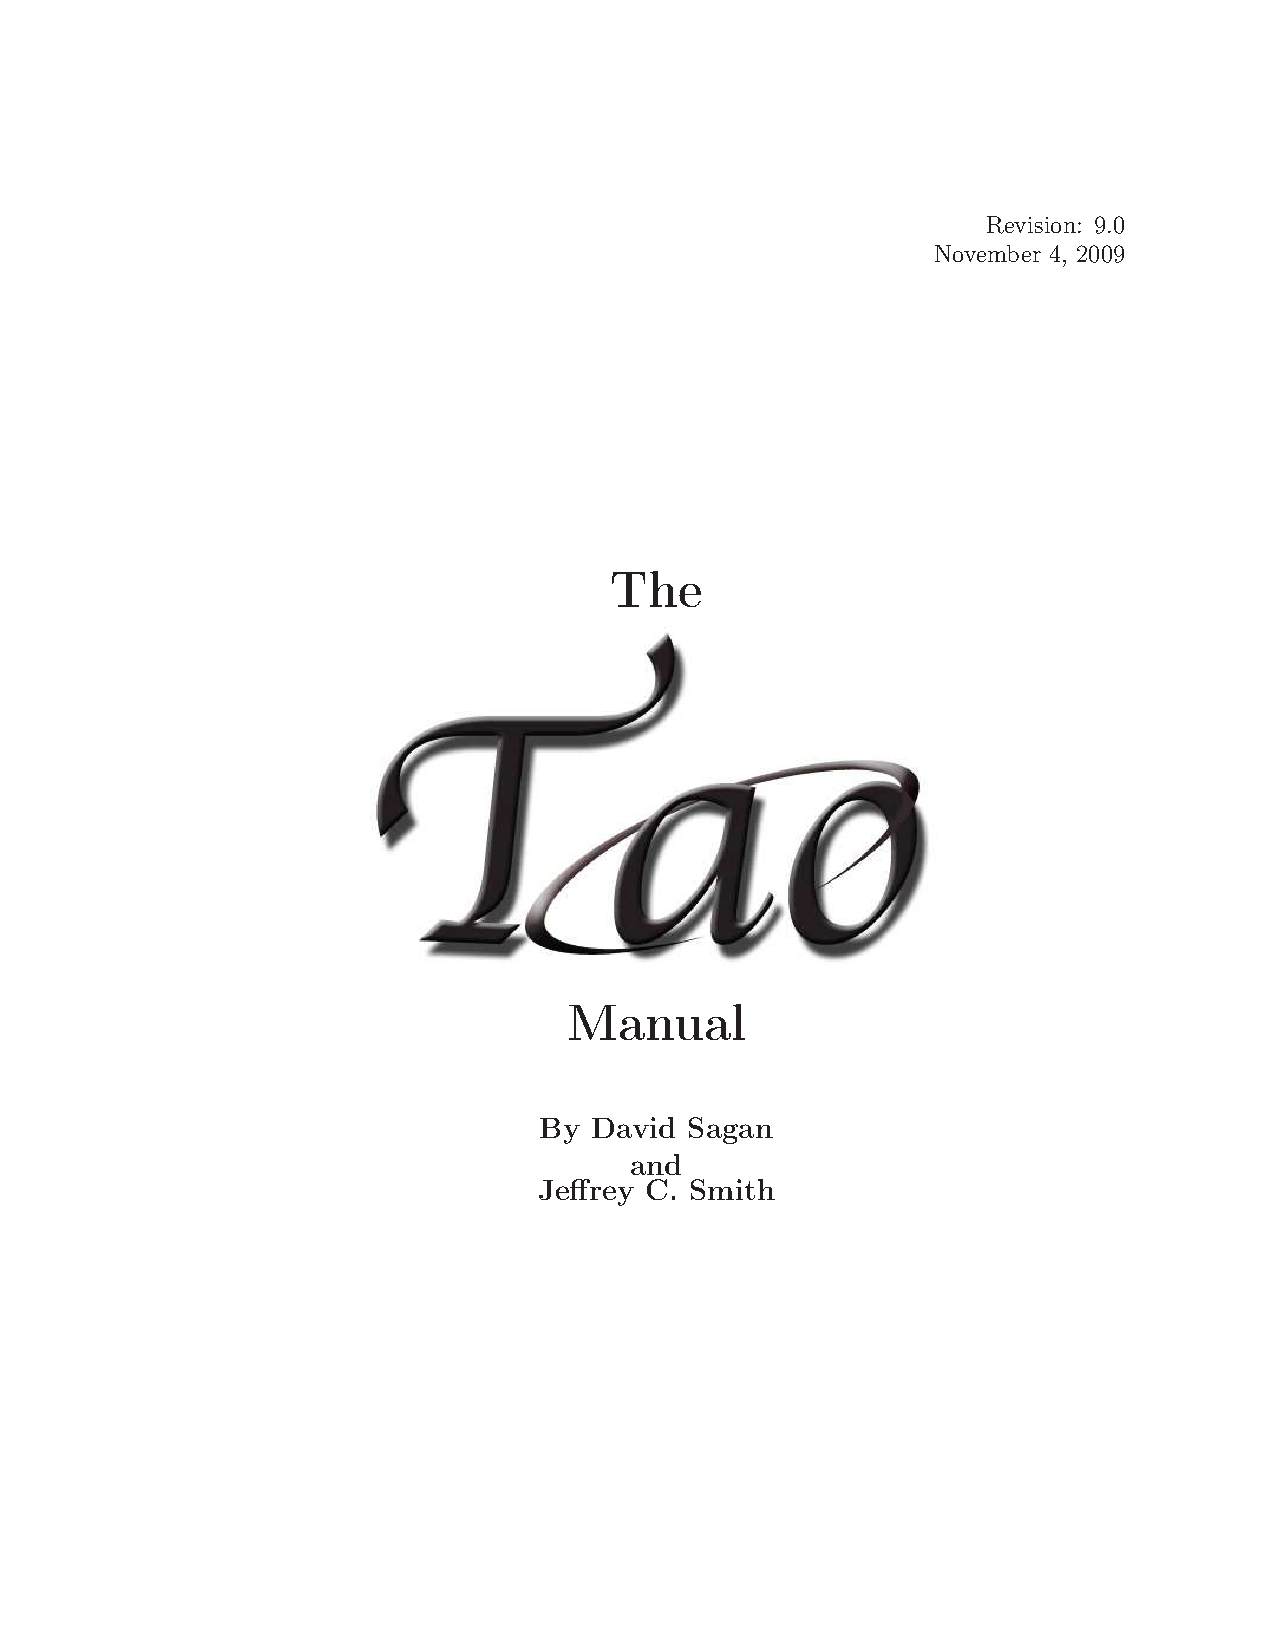
\includegraphics[width=10cm]{tao.psfig} \\
\vskip 0.1in
{\Huge \sf\bf Tutorial} \\
\vskip 0.1in
{\normalsize \sf\bf by Jeffrey C. Smith} \\
\end{center}
}

\vskip 1in
\begin{center}
{\Huge \bf *** DRAFT ***}
\end{center}
\vfill
\break
%----------------------------------------------------------------
%Introduction

{
\setlength{\parskip}{\dPar}
\setlength{\parindent}{0ex}

\section*{Tao: The Tool for Accelerator Optics}

Many simulation problems fall into one of three categories: 

\begin{itemize}
\item 
You want to design a lattice subject to various constraints.
\item 
You have some measured data and you want to make a correction. For
example, you want to know what steering strength changes will make an orbit
flat.
\item
You want to simulate what happens to the orbit, beta function,
etc., when you change something in the machine.
\end{itemize}

Programs that are written to solve these types of problems have common
elements: You have variables you want to vary in your model of your
machine, you have "data" that you want to view, and, in the first two
categories above, you want to match the machine model to the data (in
designing a lattice the constraints correspond to the data).

Because of this commonality of design, the \tao program was developed
to reduce the time needed to develop working programs. \tao is a
machine independent program that implements the essential ingredients
needed to solve simulation problems. To make the
connection, \tao uses configuration input files that can be tailored to
specific machines. Additionally, \tao has been built
to be easily customizable so that extending \tao to solve new and
different problems is relatively straight forward.

More information, including the most up--to--date version of this
tutorial, can be found at the \bmad web site at
\begin{example}
  http://www.lepp.cornell.edu/~dcs/bmad
\end{example}

Tutorials are always difficult to write. Please send any recommendations 
for imporvement or notices of outright errors to:
\begin{example}
  Jeff Smith <js344@cornell.edu>
\end{example}
}

%----------------------------------------------------------------
\tableofcontents
%% \listoffigures
%% \listoftables

\setlength{\parskip}{\dPar}
\setlength{\parindent}{0ex}

%----------------------------------------------------------------
\chapter{Before we start}
\label{c:before_beginning}

\tao is readily customizable. However beginners are advised to start with
''out of the box'' \tao while getting to know the program.

\section{Getting and Compiling \tao}

\tao is available in the \cesr CVS area. To checkout a copy type \cmd{cvs co
tao} in the directory from where you want to run \tao. If you don't have \cesr
CVS write permission then type \cmd{cesrcvs co tao}. This will check out a copy
but will not allow you to check in changes to the code. If you aren't at Wilson
Laboratory then contact David Sagan <dcs16@cornell.edu> to obtain a copy. 

From the newly created \cs{./tao} directory type \cmd{gmake -f M.tao} to create
the ''vanilla'' \tao program. Vanilla \tao is the basic \tao program without any
user customizations. this tutorial covers to basic usage of this program.
If you are using a custom version of \tao then
follow the compiling directions from the custom \tao author. Keep in mind that
command syntax and usage may vary between custom versions of \tao (this is a
\textit{feature} \textbf{not} a bug!).

Once \tao has compile go to the subdirectory \cs{./program} and type
\cmd{../../bin/tao} to run the program. This directory contains all the
configuration files to get everything working.

\subsection{customising \tao}

If you are creating a custom version of \tao then you are already more advanced than
the scope of this tutorial! See the \tao Reference Manual for details.

%----------------------------------------------------------------
%----------------------------------------------------------------
\chapter{In the Beginning...}
\label{c:beginning}

%----------------------------------------------------------------
\section{There was the the user}

This tutorial assumes the reader is already familiar with basic particle beam
dynamics and its formalism. There are several books that introduce the topics
very well. the best the author has found so far is \textit{The Physics of
Particle Accelerators} by Klaus Wille. 

\tao is based on the \bmad subroutins library and the reader is assumed to have
a working knowledge of the conventions used by \bmad. \tao can be used ''out of
the box'' so an understanding of the nitty-gritty details of \bmad is not
necessary, however, one should be familiar with the material in chapters 1 and 2
of the \bmad manual.

\fbox{introduce the basic things one would want to do with \tao}

This tutorial is designed to get the user up and starting with \tao without
needing to dredge through the entire reference manual. Full command syntax
or greater detail on any topic can be found in this manual.

%----------------------------------------------------------------
\section{Then there was the super-universe}

Everything known to \tao is placed in an area called the
\textit{super-universe}. Within the \textit{super-universe} lies one or more
universes each containing a particular machine lattice. This allows for the user
to do analysis on multiple machines or multiple configurations of a single
machine at the same time. 

\subsection{A typical universe}
A universe contains a \bmad lattice plus whatever data one wishes to study
within this lattice (i.e. twiss parameters, orbit, phase \&etc...\. Actually,
there are three lattice instances within each universe: the \textbf{design
lattice}, \textbf{model lattice} and \textbf{base lattice}. All lattice changes
specified during a session are incurred on the model lattice. The design lattice is
fixed at initilization time and serves as a reference point for any elemental
changes incurred during the \tao session. The base lattice also serves as a
reference point but the user can transfer the model lattice over to the base
lattice whenever it is desired.

Each data point (for example, the horizontal orbit at some detector) has 5 datum
 quantities associated with it: the \textbf{measured data}, \textbf{reference
data}, \textbf{model data}, \textbf{design data} and \textbf{base data}. The
model, design and base data areas correspond to the appropriate quantity
calculated in their respective lattice above. The measured data corresponds to 
data obtained during a measurement. If doing design work then the desired data
value would be placed here \( this is also refered to as a constraint during
optimization\). The reference data is just like the base data except it isn't
associated or synchronized with a lattice.

\subsection{Variables}

Variables control attributes of elements in the model lattice of one or more
universes. So, a given variable may control a single atribute of one element
for one or more universes. 

\subsection{Other stuff in the Superuniverse}

The super-universe also contains information pertaining to global variables and
plotting. The the \tao referenc emanual for details.

%----------------------------------------------------------------
%----------------------------------------------------------------
\chapter{Getting information from \tao}
\label{c:get_info}

%----------------------------------------------------------------
%----------------------------------------------------------------
\chapter{Modifying the lattice}
\label{c:modify_lattice}

%----------------------------------------------------------------
%----------------------------------------------------------------
\chapter{Running the optimizer}
\label{c:optimizer}

%----------------------------------------------------------------
%----------------------------------------------------------------
\chapter{Single Mode}
\label{c:single_mode}

%----------------------------------------------------------------
%----------------------------------------------------------------
\chapter{Where to go from here}
\label{c:where_to_go}

\end{document}
